\documentclass{article}
\usepackage[utf8]{inputenc}
\usepackage{tikz}
\usetikzlibrary{positioning}
\begin{document}
	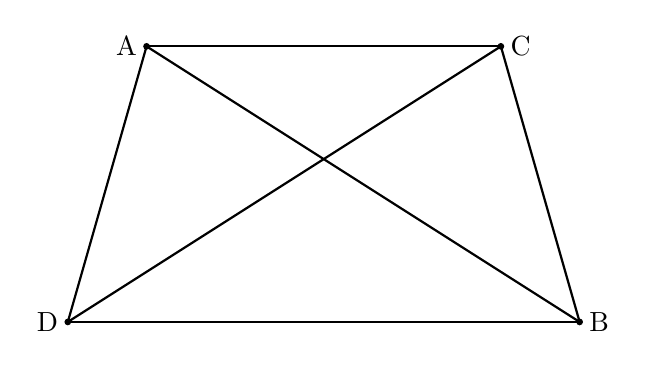
\begin{tikzpicture}
    	\draw[black, thick] (0,0) --(1,3.5); 
	\draw[black, thick] (1,3.5)--(5.5,3.5);
	\draw[black, thick] (5.5,3.5)--(6.5,0);
	\draw[black, thick] (6.5,0)--(0,0);

	\draw[black, thick] (0,0)--(5.5,3.5);
	\draw[black, thick] (1,3.5)--(6.5,0);
	
	\filldraw[black] (0,0) circle (1pt) node[anchor=east] {D};
	\filldraw[black] (6.5,0) circle (1pt) node[anchor=west] {B};
    	\filldraw[black] (5.5,3.5) circle (1pt) node[anchor=west] {C};
    	\filldraw[black] (1,3.5) circle (1pt) node[anchor=east] {A};
	\end{tikzpicture}
\end{document}
